% flotsam.tex
%
% Predrag created file				jun 20 2006

\section{Flotsam}


\subsection{KS box {\rpo s}}

Davidchack and Crofts found that full space KS $L = 22.0$, 
appears to be the smallest $L$ with persistent chaos.  
, $L=22$ is a good choice because in units of mean wavelength
this is about $ \tilde{L}/\sqrt{2}= 2.4758$
2.5 wavelengths, so the 
dynamics in this small system is competition between wavenumbers
2 and 3. 2-equilibrium and the 2(?) 3-equilibria essentially lie in
the 2nd and 3rd Fourier component complex planes, respectively, with very
small deformations from higher harmonics.


\subsubsection{Equilibrium A}

Equilibrium A eigenvalues of $\Mvar$:

$(\Lyap_i \pm \theta_i)
=(
  0.13903973 \pm i 0.23842023,
 -0.08402656 \pm i 0.16019413,
 -0.11941393, 
 -0.27112264 \pm i 0.35630716,
 -2.01303043,
 -2.03775342,
 -5.63649418,
\cdots
)$

This equilibrium has no symmetric partner SA (it is selfdual?).

\ES{I observe pairs of real eigenvalues,
e.g. -58.3602685 and -58.3602681. As their absolute
value increases they differ even less.
I think it has to do with the linear part being the main
contribution to $\Mvar$ for higher modes, as well as 
with treating real and imaginary components 
as separate variables, which means it will appear twice.
\\
PC: I think such contracting eigenvalues as -58.3602685 have no meaning.
Even if they are accurate eigenvalues of $\Mvar$,
by the time you compute
$\ExpaEig_{radial} =  e^{\Lyap_p \period{p}} = e^{26\cdot58} = e^{1510}$ you got
computationally a serious underflow.
}

The equilibrium point is accurate to at least to $10^{-11}$. Since
Lapack is also double precision accurate, the accuracy of the first
few eigenvalues is similar, and certainly in
excess of 6 significant digits.



For a numerical check of the \rpo\ stability eigenvalues,
used two inital
points along an unstable eigenvector $\jEigvec{1}$
at radial distance  $\approx 10^{-4}$ from the equilibrium A,
and the initial inter-point separation $\Delta(0) \approx 10^{-5}$.
Integrated for time equal to the period $\period{p}=26.3556$ as calculated from
the \jacobianM\ and computed the leading Lyapunov exponent from the ratio of
final to initial distance 
$\Lyap= {1 \over \period{}}\ln( \Delta(\period{})/\Delta(0))$.
Get
$\Delta(\period{})/\Delta(0) =39.01$,
$\Lyap=0.13902$, in agreement with the equilibrium point A 
expanding eigenvalue $\Lyap=0.13904$
\[
\ExpaEig_{radial} =  e^{\Lyap \period{}} =38.99
\,.
\]

\underline{Need to trace out}
the unstable manifold plane, like Gibson did for plane Couette.
You compute the 2 expanding eigenvectors of the
equilibrium A, as well as the 3rd, least contracting direction; then
translate and rotate your Fourier modes into this coordinate frame,
and plot the trajectory there, both in the lab and the co-moving frame.

Vaggelis proved this statement wrong:
By symmetry there might be an equilibrium on the reflection plane that
relates the equilibrium A and its symmetry partner SA; the 3 equilibria would
be analogous to what you see in the Lorentz attractor pictures, crossing
the unstable manifold of the central one throws you into the neighborhood
of the other equilibrium.

\underline{Next step}: try to find the equilibrium that corresponds to fitting
exactly 3 complete periods of $u(x)$ into interval $L$.
Orbits coming close to this one
show up in Davidchack's \rpo s.

\subsection{\Reqva}

\underline{Need to determine} important {\Reqva} (traveling waves).

The \reqva s (or travelling waves) have a limiting propagation
velocity $d/\period{}$. To visualize it numerically,
start with a $\delta$-function
shaped $u(x,0)$, or, in Fourier space, with all Fourier coefficients real
and equal. Time evolution of this  $u(x,t)$ consist of two constant 
velocity pulses.

Determine their velocity ANALYTICALLY.

\subsection{\Rpo s}

\ES{
The names of the \rpo\ figure files follow the convention
 {\tt rpoL-T-d.eps}s, with suffixes {\tt cm}
and {\tt u} indicating
 co-moving frame  and $u$ representation respectively.
   }
%
Davidchack and Crofts 
investigate this sytem in 15 modes (30-dim system of ODEs) truncation.
Out of 30 \rpo s they
find,  only three are truly periodic.  The orbit
with $\period{p} = 95.25$ has a very small
$d = -6.5\,e^{-7}$, but it is not periodic 
(they
checked this by decreasing the integration step size and increasing the
number of modes).

The dynamics in this small system is competition between wavenumbers
2 and 3. The 2-equilibrium and the (2?) 3-equilibria essentially lie in
the 2nd and 3rd Fourier component complex plane, with very
small deformations from higher harmonics.
Hence plot all \rpo s in these 2 representations:

$[ \Re a_2, \Im a_2, \Re a_3 ]$
(here 2-equilibrium is a circle, 3-equilibrium (-ia?) a vertical line)
 and
$[ \Re a_3, \Im a_3, \Re a_2 ]$
(here 3-equilibrium is a circle, 2-equilibrium a vertical line)

It is very instructive, and seems to suggest that some as yet
undetermined travelling waves control most trajectories part way.

The \rpo\ [NAME IT] travels between the equilibrium A and a
travelling wave B (?) 
with period and shift
$\period{p}=55.5953 d=5.24725$
Compared to $L/4 = 5.5$
this is nice, but why not close to periodic after 2nd return? Why 4th return?

[NAMEIT] \rpo\ looks similar to Davidchack's  orbit
of period 
$\period{p}=47.64$ and $d=5.6759$. The period appears to depend on how
many times the orbit manages to spiral around the equilibria.
For [NAMEIT] that appears to be
1.5 times per period, rather than 2. This would led as
to
think there is a family of \rpo s along with a 3rd unit eigenvalue of
$gJ$,
but such does not exist.
So there has to be a selection mechanism corresponding to
reaching or missing the neighborhood of an equilibrium point starting from
the neighborhood of the other. 

This stuff is hard to visualize... for ordinary periodic orbits one
plots the unstable plane of the equilibrium, shows where the periodic
orbits sit.

Better visualization is in co-moving frame, {\ie} 
a reference frame that translates with with velocity $d/\period{p}$.
In the co-moving frame a \rpo\ becomes
a \po.
Co-moving frmae visualization helps quite a bit. Put a black (green, respectively) dot
twice thicknes of the line every time unit; it will enable you to see
where the motion is slow and where it is fast
% (a trick we used to understand plane Couette trajectories).
Mark the inital point on both
co-moving rpm and on equilibrium in co-moving frame with a fat triangle
indicating the direction, so we can see how they both move. Probably at the
opposite ends of the two curves - co-moving frame is the mean motion.

Each {\rpo} has its own co-moving frame - and within it, equilibria
move on circles (or worse - because in higher Fourier modes they do mmore
complicted things), and it is important to know where the equlibrium is at
a given instant.

The $u$ space time evolution \reffig{f:rpoNAMEITu} % rpo22-55-4-u.eps 
is plotted with the same starting instant,
so one can also track also the spatial profile $u$ in parallel with
the Fourier space projections.

So it is almost impossible to see \reffig{f:rpoNAMEIT}(b) %rpo22-55-4-cm.eps
in \reffig{f:rpoNAMEIT}(a) % rpo22-55-4.eps.
I can see 4 periods in \reffig{f:rpoNAMEIT}(a), %po22-55-4.eps,
but not in \reffig{f:rpoNAMEIT}(b) %rpo22-55-4-cm.eps
where it comes back only after full period $\period{p}=55.6$.

It still seems that it could be made relative periodic 
(modulo a reflection symmetry?)
in $\period{p}/4=55.6/4=13.9$? That would be OK 
-
by symmetry the figure 8 connecting
2 symmetric equilibria could consist of 4 identical segments: from
equilibrium A to midplane, then reflected version of the same to SA, and
back again.


%%%%%%%%%%%%%%%%%%%%%%%%%%%%%%%%%%%%%%%%%%%%%%%%%%%%%%%%%%%%%%%%
\begin{figure}[t] %[h]
\centering
 	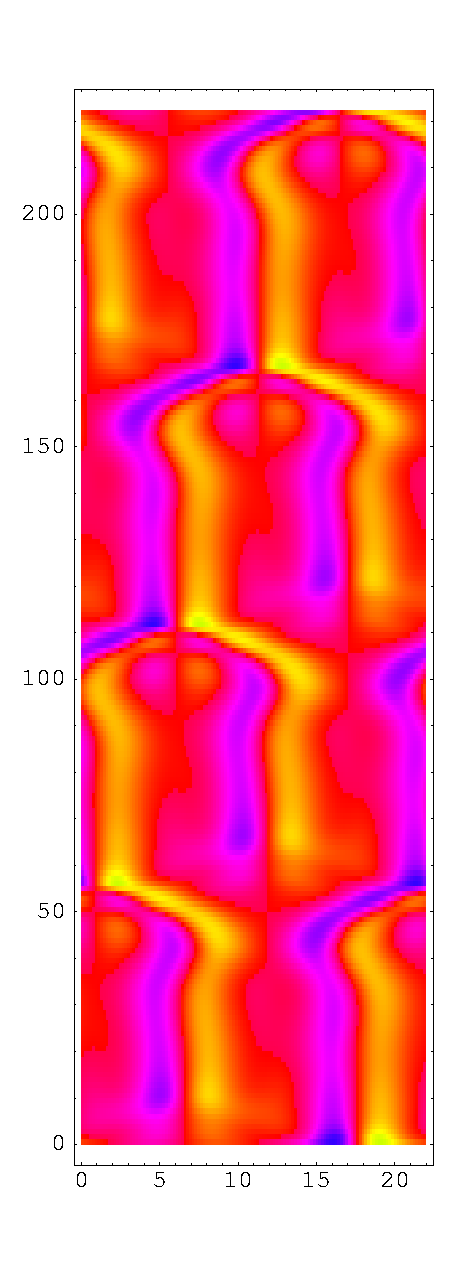
\includegraphics[width=2.5cm]{figs/rpo22-55-4-u.eps}
\hspace{0.1in}
\caption{
 The \rpo\ [NAMEIT] in $u(x,t)$ representation. 
        }
\label{f:rpoNAMEITu}
\end{figure}
%%%%%%%%%%%%%%%%%%%%%%%%%%%%%%%%%%%%%%%%%%%%%%%%%%%%%%%%%%%%%%%%%%


%%%%%%%%%%%%%%%%%%%%%%%%%%%%%%%%%%%%%%%%%%%%%%%%%%%%%%%%%%%%%%%%
\begin{figure}[t] %[h]
\centering
(a) 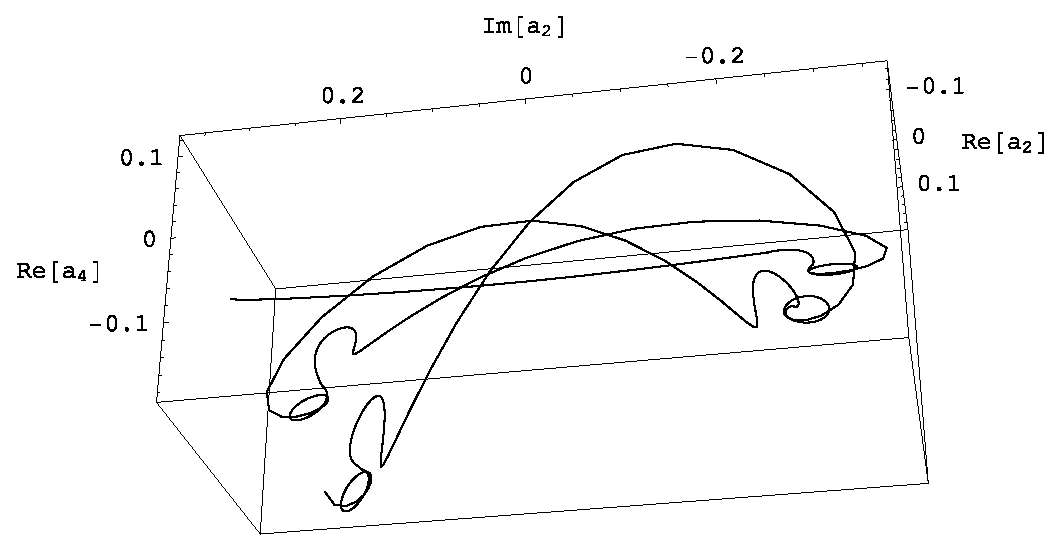
\includegraphics[width=8.0cm]{figs/rpo22-55-4-clean.eps}
% ./removecache.sh rpo22-55-4.eps
% abandoned rpoEq22-55-4.eps with co-moving equilibrium embeded.
%
\hspace{0.1in}
(b) 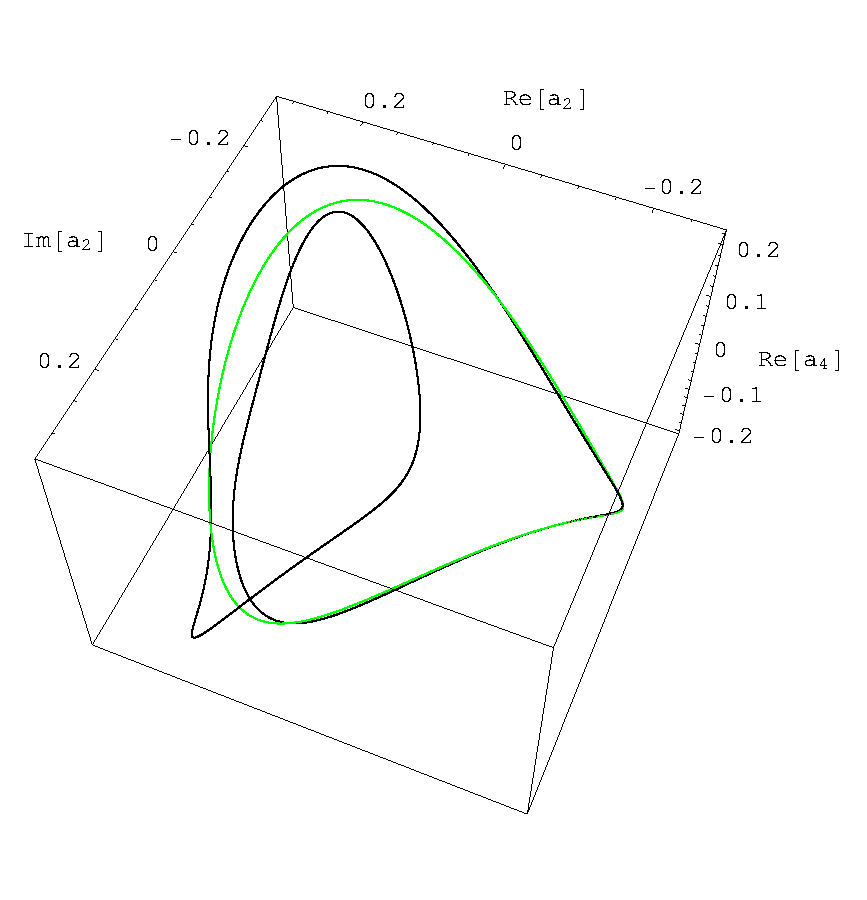
\includegraphics[width=6.0cm]{figs/rpoEq22-55-4-cm.eps}
\\
(c) [create rpoEq22-55-4-cm-?.eps]
\caption{
 The \rpo\ [NAMEIT] in: 
 (a) Phase space, traced for four periods $\period{p}$.
% Green curve belongs to \reffig{f:rpoNAMEIT}(b) % rpo22-55-4-cm.eps
% rather than to  \reffig{f:rpoNAMEIT}(a), % rpoEq22-55-4.eps?
 (b) co-moving frame. 
        The continuos family of 
	equilibria A obtained by the action of $g$ is shown in green,
	the SA family shown in red. The \rpo\ [NAMEIT] stays close
	to either A or SA for close to 1/2 of equilibrum rotation
	period, then quickly jumps to the other equilibrium point.
 (c) co-moving frame A, SA and [NAMEIT] projected on the 
	$[a_?,a_?]$ plane,
	with the $\sigma x = -x$ symmetry of \KSe\ explicit.
        }
\label{f:rpoNAMEIT}
\end{figure}
%%%%%%%%%%%%%%%%%%%%%%%%%%%%%%%%%%%%%%%%%%%%%%%%%%%%%%%%%%%%%%%%%%


The two equilibria
capture qualitatively the co-moving frame \rpo\ [NAMEIT] shape,
which follows the
equilibrium for most of the time, except for a quick swing where it
sidesteps by $d/4$, just as it does in \reffig{f:rpoNAMEIT}. 

Please also plot it in plane, chose small Fourier coefficients
 which respect the $x \to -x$ symmetry of \KSe.
Then the symmetry of 2 co-moving
equilibria and self-dual symmetry of \rpo\ [NAMEIT] will be explicit.

Eigenvalues of \rpo\ [NAMEIT] $g\jMps$: are
$ -57.17,  1.00009, 1.00001, -0.500, -0.012, \cdots$ .
%
%  Eigenvalues of the Jacobian without rotation
%  84.15, -33.86 + 28.94 i, c.c. , 0.48, 0.00019
% no good - missing marginal ones

Predrag wrong here:
This all makes sense: The period is roughly double of the rotation period of
the equilibrium point, as the trajectory makes a figure 8 around equilibrium A and
its symmetric partner SA.

 There are two
marginal eigenvalues, one for time translation, one for
circle translation. 
The sign of $\ExpaEig_{1}=-57$ says this is a Moebius-kind orbit,
inverse hyperbolic, presumably due to the symmetry relating A and SA.
Lyapunov $\Lyap=0.07$ says that this neighborhood is much less repelling than
the central equilibrium A, a better candidate for being embedded into the
ergodic attractor.

The \rpo\ initial condition is
so accurate the orbit in \reffig{f:rpoNAMEIT}(b)
start visibly deviating after retracing the loop 6.5 times.
% the largest unstable multiplier is 
% $-57.17$ per period of the orbit - error would grow to $\approx 60^7
% = 2,800,000,000,000$.

For the \rpo s the accuracy of Jacobian depends
on the time step size, and long runs are needed to refine the results
We check by redoing the calculation with double 
number of Fourier modes, observe how many digits
change. 
Because of the strong contractionin KS we expect at most 10 eigenvalues to be
significant, rest are in the numerical noise. See figure~6 in
\refref{Christiansen:97}.
Stated here are only the digits we trust.

